\documentclass[12pt, a4paper]{article}
\usepackage[utf8]{inputenc}
\usepackage[noconfigs, english]{babel}
\usepackage{graphicx}
\usepackage{url}
\usepackage{subfig}
\usepackage{multicol}
\usepackage{float}
 \setlength{\columnsep}{1cm} 

\pagenumbering{arabic}
\bibliographystyle{unsrt}
  
\usepackage{natbib}


\usepackage[pdftex,
            pdfauthor={Abbas Bushehri, Chisom Kobbe-Nwabufo, Florian Kessler, Lukas Heimann, Rahul Tak, Syed Habibullah},
            pdftitle={Team-Oriented Project Documentation},
            pdfsubject={Project Documentation},
            pdfkeywords={team-oriented project, facial recognition, opencv},
            pdfproducer={Latex Texmaker JabRef},
            pdfcreator={pdflatex}]{hyperref}


\title{Team-Oriented Project}
\author{Abbas Bushehri, Chisom Kobbe-Nwabufo, Florian Kessler,\\
	Lukas Heimann, Rahul Tak, Syed Habibullah \\
	University of Applied Sciences Ulm  \\
	Bachelor Computer Science 
	}

\date{\today} 

\begin{document}
\maketitle




\newpage



\tableofcontents



\newpage

\section{Motivation and Project Goal}
\subsection{Motivation}
For our team-oriented Project we wanted to evaluate if facial recognition technology would be applicable to register the attendance of students in mandatory courses. Our idea was to create a software that works as a digital attendance list. Usually when there is a mandatory course, the professor will pass around a list where everyone has to sign that they attended the lecture. However, this approach has some disadvantages for the students as well as for the professor. First of all, students could forget to sign the list. Also, this approach is prone to cheating as students can just sign the list for someone else, too. But there are also disadvantages for the professor. They have to manually enter the data on a computer and check if students attended every lecture. These Problems could impact the students motivation and grades while they also cause more work for the professors. 

\subsection{Goals}
Our idea of creating a facial recognition software that detects and recognizes students in the lecture room would solve these problems by creating the list at the end of the lecture and marking all students that it recognized as attended. An additional advantage of this software would be that we automatically show the names of all the students sitting in the classroom in the camera feed. This helps the professor to remember the names of students and can help to create a more comfortable learning environment for the students. The goal of our project was to create a proof of concept that shows that this idea could be used as an alternative to the attendance list on paper that is currently used. The software could also be improved to save more detailed statistics about the students attendance. 



\newpage



\section{Requirements}
\subsection{Functional Requirements}
There are certain fuctions our software should have at the end of the project. First of all it should be able to capture a live feed from a camera connected to the computer. Then it should have a fullscreen window that shows this camera feed. The images recorded by the camera should be proccessed by a face detection and face recognition algorithm. We want to store the training images of the students in a database. If the algorithm recognizes a student from the database we want to show their name in the camera feed. In the fullscreen window there should also be a info panel that shows important informations for the professor e.g. the number of attending students and also a list of missing students. There should be a recognization threshold (how many times does a student have to be recognized until they are marked as attended). The professor should be able to manually add students to the database. There should also be an option to select the camera which will be used. Also, there should be an option to delete certain students from the database. Furthermore we need an option to change the recognization threshold. 

\subsection{Non-Functional Requirements}
\begin{itemize}
\item Windows 10
\item VisualStudio C\# 2019
\item connectable camera with full hd resolution
\item OpenCV
\item EmguCV
\end{itemize}



\newpage



\section{User View}
When the user runs the UniFCR program, they're greeted with four buttons in the main menu as seen in figure \ref{fig:menu}:
\begin{figure}[h!]
	\centering
		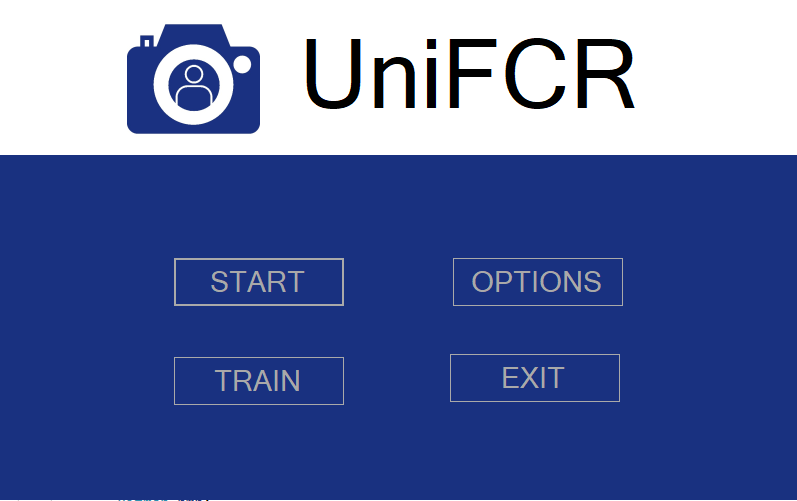
\includegraphics[width=1.0\columnwidth]{images/menu}
	\caption{Main menu of the program}
	\label{fig:menu}
\end{figure}
\subsection{OPTIONS button}
First there is the OPTIONS button. This is meant to be used to change some of the settings of the program. As shown below in figure \ref{fig:options} there are three options that can be changed:
\begin{itemize}
\item There is a drop-down list for selecting the camera. This should include the PC’s camera (if it exists) and any currently connected webcams. If a camera is connected after the program is opened it will not be shown in this list. It would only be shown after the program is opened again. 
\item There is a slider for the threshold. The threshold defines the number of times a face should be recognized before that student is marked as attended. By default, the threshold is 30.
\item There is a text box next to a DELETE button. If a student’s matriculation number is written and the button is pressed, then the student will be deleted from the database.
\end{itemize}

\begin{figure}[h!]
\begin{center}
	\centering
		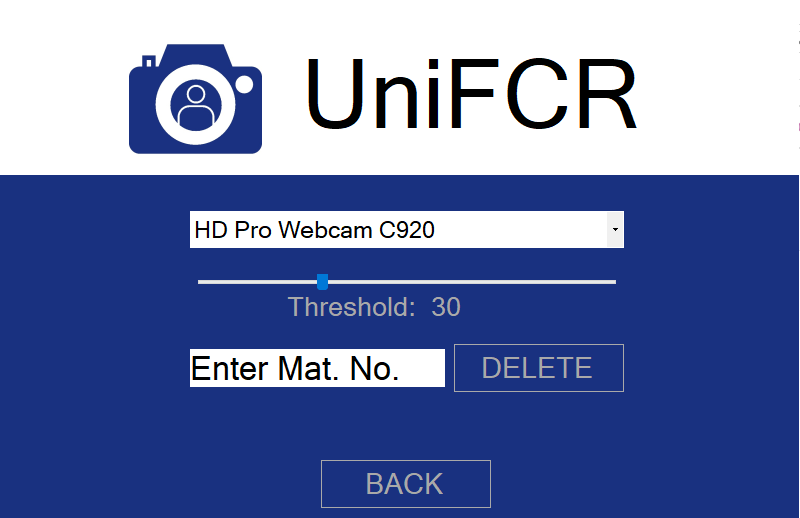
\includegraphics[width=1.0\columnwidth]{images/options}
	\caption{Options menu}
	\label{fig:options}
\end{center}
\end{figure}

\subsection{TRAIN button}
Next there is the TRAIN button. This button opens the training mode that should be used to add a student to the database. This mode implements face detection to help the student take pictures correctly, as shown in figure \ref{fig:train}. When the CAPTURE button is pressed, the camera takes ten pictures of the user. The user won’t be able to do anything until the camera is finished taking these pictures. The user can press the CAPTURE button multiple times to make sure they will have more pictures in the database. When the user is satisfied with the amount of pictures they have taken, they should make sure that their name and matriculation number has been written into the text boxes. Then the user should press the SAVE button. This will add all the student’s data to the database. If the text boxes were not filled up an error will be thrown. When done the user can press BACK to return to the main menu.
\begin{figure}[h!]
\begin{center}
	\centering
		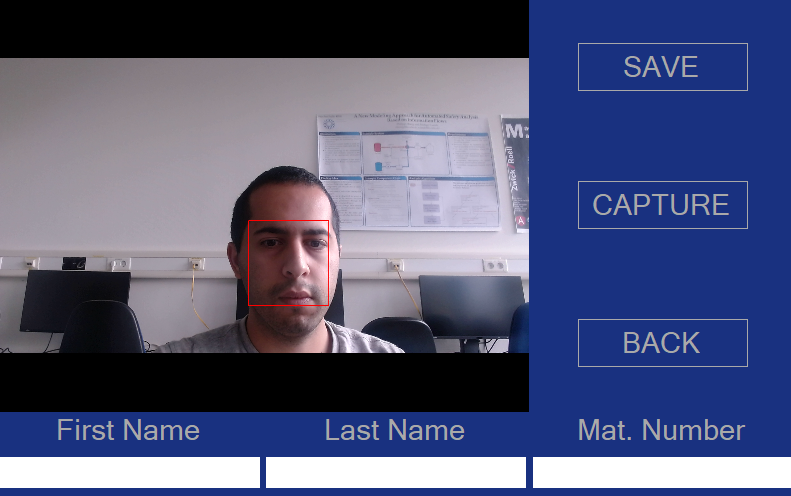
\includegraphics[width=1.0\columnwidth]{images/train}
	\caption{Training mode}
	\label{fig:train}
\end{center}
\end{figure}

\subsection{START button}
The next button is the START button. This opens the attendance mode. Attendance mode implements face recognition. The name of the user is written on top of the rectangle that marks the detected face. On the right side there is a percentage counter that keeps track of the percentage of students that have been marked as attended. Below that is a list of all the student in the database. If a student is marked as attended then their name is highlighted blue. Figure \ref{fig:before} shows before the student is marked as attended, and figure \ref{fig:after} shows it after the student is marked. The user can press the BACK button to return to the main menu.  

\begin{figure}[H]
  \centering
    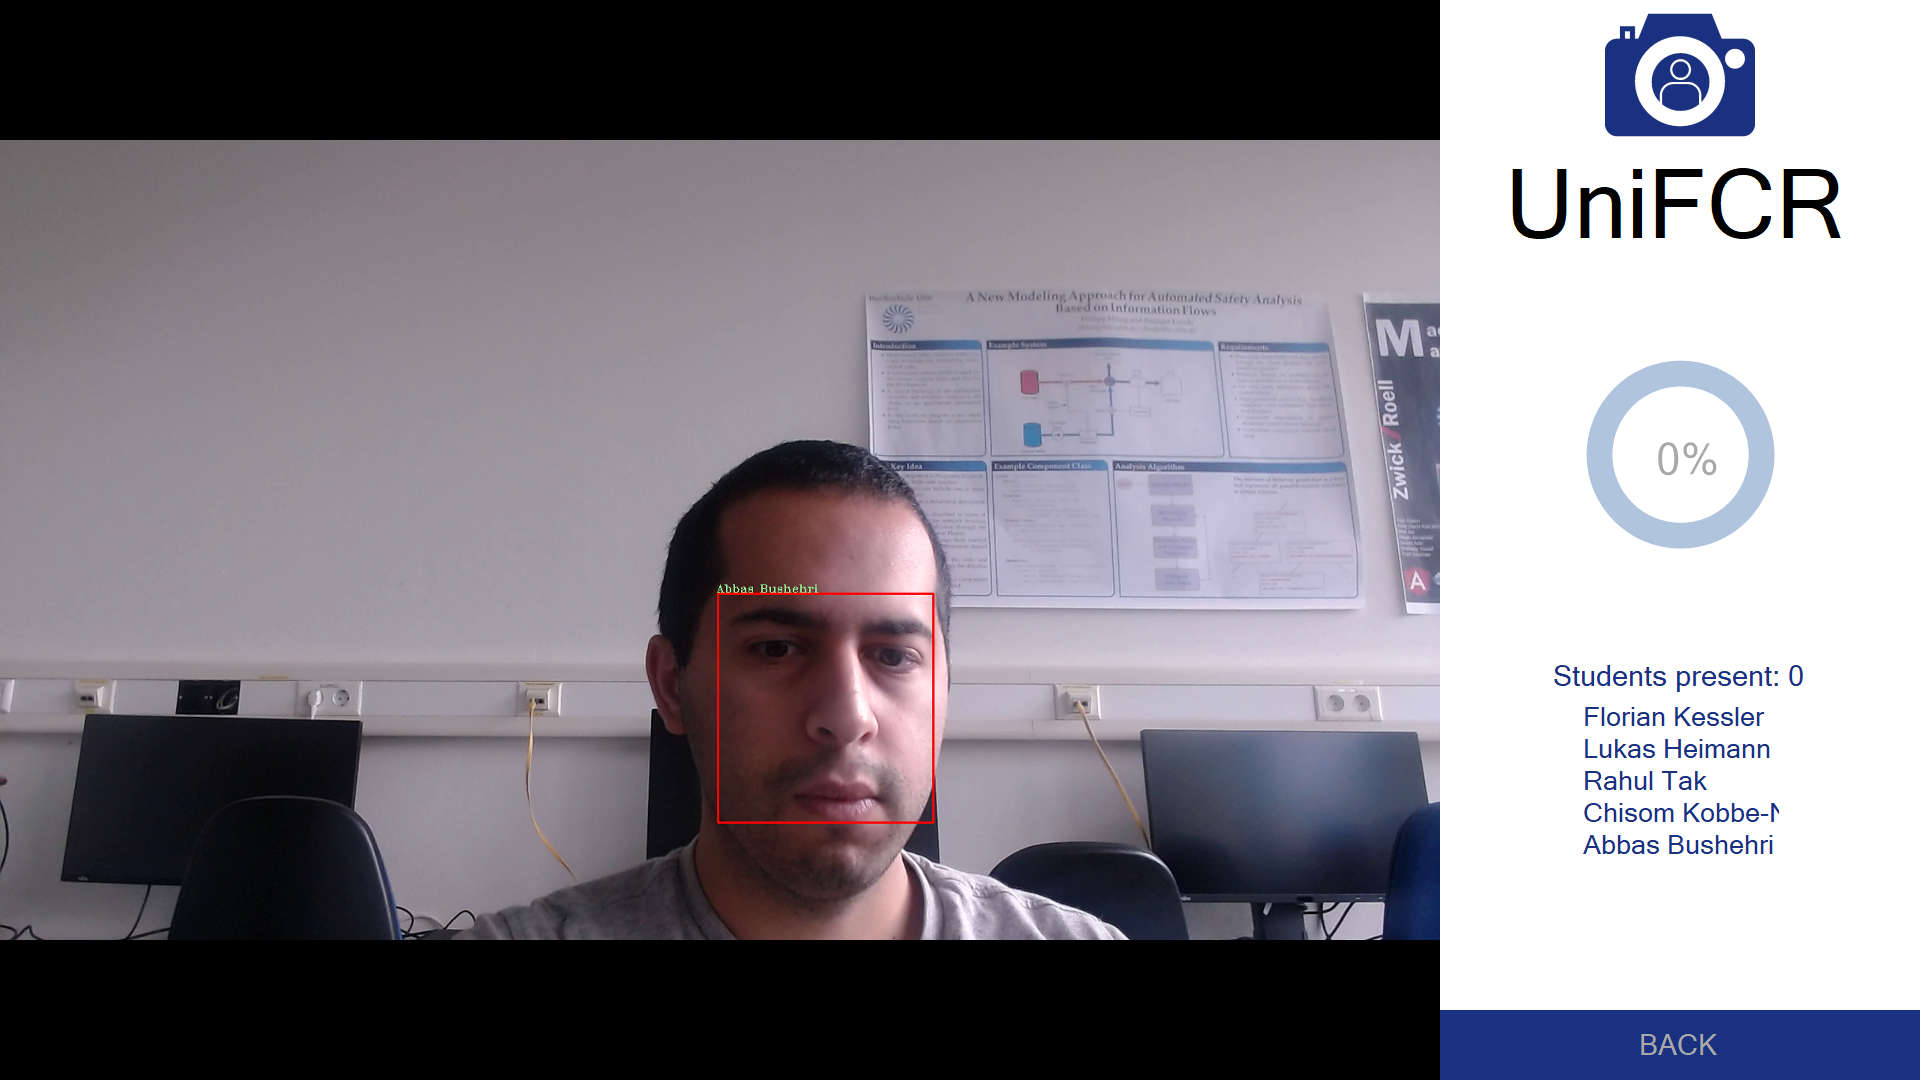
\includegraphics[width=1.0\textwidth]{images/before}
    \caption{Attendance mode when it starts}
    \label{fig:before}
  \end{figure}

 \begin{figure}[H]
    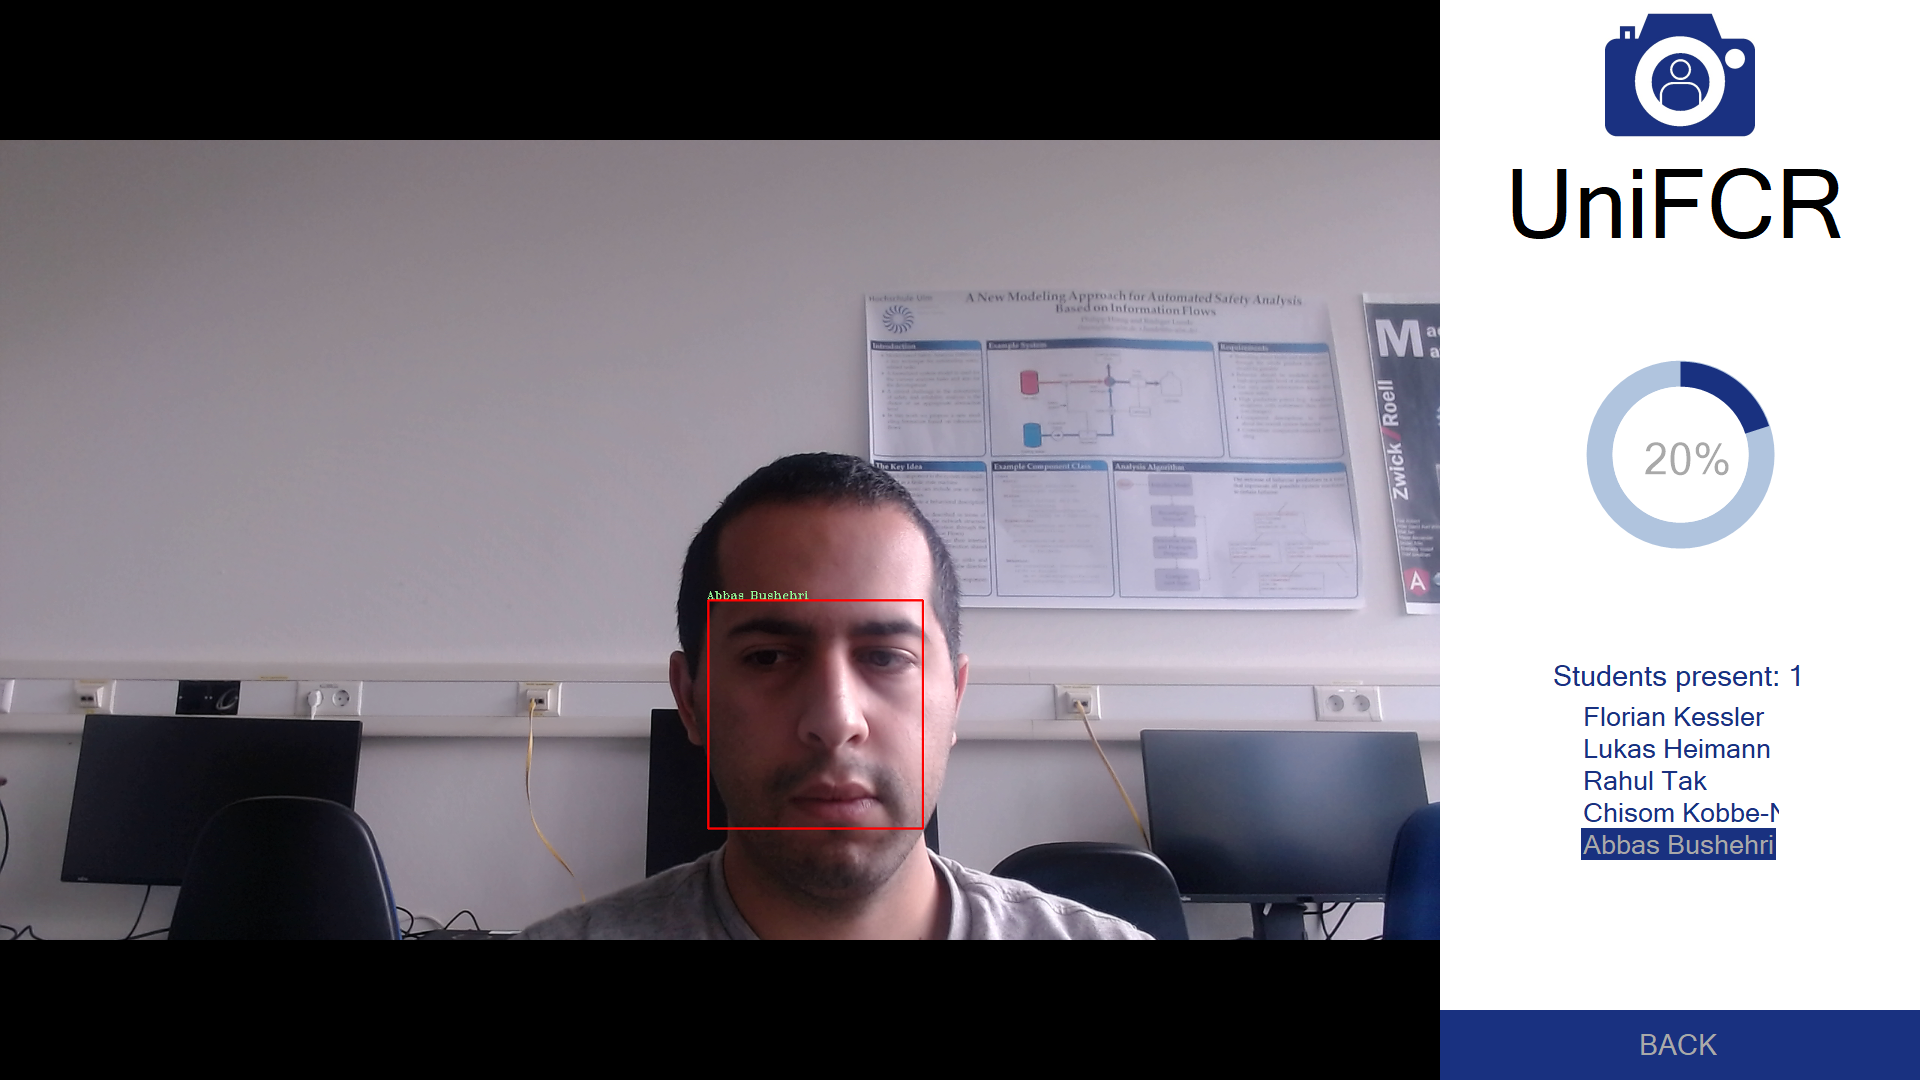
\includegraphics[width=1.0\textwidth]{images/after}
    \caption{Attendance mode after a student has been marked as attended}
    \label{fig:after}
 \end{figure}

\subsection{EXIT button}
Finally the main menu has the EXIT button. This closes the program. Before the program is closed, a pop-up window asks the user if they want to save the attendance list (figure \ref{fig:popup}). If the user presses yes, then a .csv file is created in a Lists folder as shown in figure \ref{fig:folder}. The file is named after the current date, and lists all the student’s data along with whether or not they were marked as attended, as shown in figure \ref{fig:csv}.
\begin{figure}[h!]
\begin{center}
	\centering
		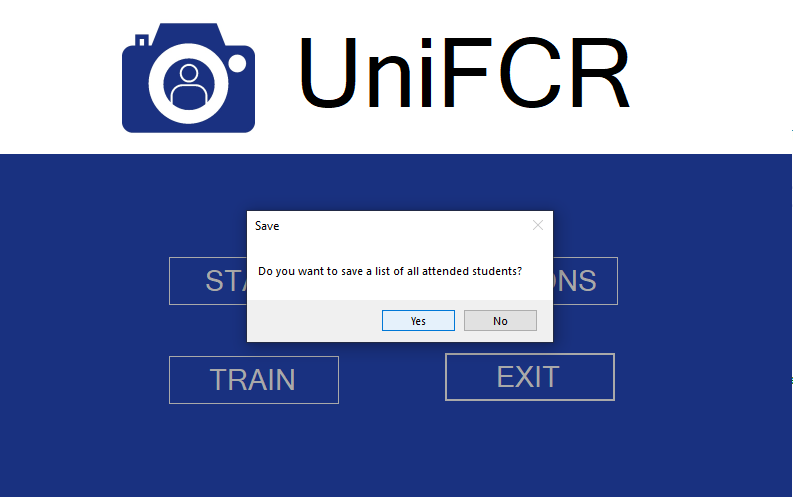
\includegraphics[width=1.0\columnwidth]{images/popup}
	\caption{Pop-up window appears after user tries to exit}
	\label{fig:popup}
\end{center}
\end{figure}
\begin{figure}[h!]
\begin{center}
	\centering
		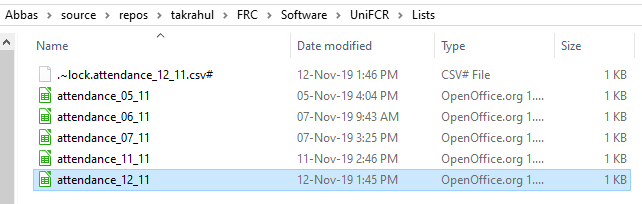
\includegraphics[width=1.0\columnwidth]{images/folder}
	\caption{Attendance lists saved in the Lists folder}
	\label{fig:folder}
\end{center}
\end{figure}
\begin{figure}[h!]
\begin{center}
	\centering
		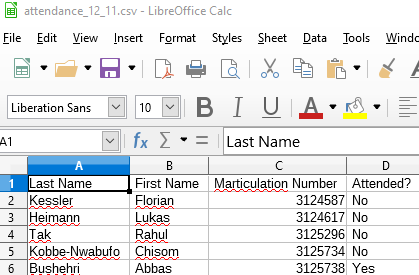
\includegraphics[width=1.0\columnwidth]{images/csv}
	\caption{Contents of an attendance list}
	\label{fig:csv}
\end{center}
\end{figure}
\subsection{Loading screen}
Whenever the program is loading after the TRAIN or START buttons are pressed, the following image is shown as a loading screen. The loading screen is shown in figure \ref{fig:load}.
\begin{figure}[h!]
\begin{center}
	\centering
		
\includegraphics[width=1.0\columnwidth]{images/load}
	\caption{Loading screen image}
	\label{fig:load}
\end{center}
\end{figure}



\newpage




\section{Technical Concenpt}
\subsection{OpenCV Explanation}
OpenCV is a library of programming functions aimed at computer vision. This means it can read images, write images, and detect objects in images. In the case of this project, OpenCV is needed for its facial detection and recognition capabilities. This project is written using C\#, which OpenCV does not support. However, there is Emgu CV which is a .Net wrapper for OpenCV. This means Emgu CV can be used for programming in C\#. During the project the following methods and functions were used from the Emgu CV library:
\subsubsection{Image}
The Image object will be used for either storing the frame that is captured by the camera, the frame that will be shown to the user in the GUI, or a cropped view of a face that has been detected.  In Emgu CV the Image object is defined by the two generic parameters color and depth. We need the image to be gray-scaled with a depth of one byte for the algorithm to work. When we use the Image object for the camera frame it should not be gray-scaled. So we use \textit{Image\textless Gray, byte\textgreater} for storing the faces and \textit{Image\textless Bgr, byte\textgreater} for storing the camera frame. The Image object comes with many functions including:
\begin{itemize}
\item Convert(): This method converts an image into a different color and depth. This is method is used for converting the frame’s Image\textless Bgr, byte\textgreater into Image\textless Gray, byte\textgreater for the facial detection and recognition algorithms, and also for converting it back. It is also used to convert a Rectangle object, that was returned from the face detection, into an Image\textless Gray, byte\textgreater.
\item Resize(): This method is used to resize the Image object. We use it to make sure all the Images of faces we take have the same size (100 pixels for both width and height). We also use it for setting the size of the Image the user sees in the GUI.
\item Copy(): Used to copy an Image object from one variable to another.
\item EqualizeHist(): Used to normalize the brightness and contrast of an Image. We used it for the Images that store the faces to improve algorithm accuracy.
\item Draw(): Used to draw a rectangle of specified color and thickness. We used it to draw a red rectangle (with thickness of 2) surronding the detected faces.
\end{itemize}
\subsubsection{CasscadeClassifier} The CasscadeClassifier class is used for object detection. In our case, we use it for face detection. When a CasscadeClassifier object is initialized with a file (typically an xml file) that stores the classifier values. These classifier values depend on the type of object that is to be detected. We used an xml file from the internet. After the CasscadeClassifier is initialized, we only used one of the object’s methods:
\begin{itemize}
\item DetectMultiScale(): This method returns an array of Rectangle objects that stores all the objects detected that match the classifier values. In our case it returns a Rectangle array of faces. The parameters of this method include the Image object it should scan, which is the frame from the camera. We can also set the minimum and maximum size of a detected object.
\end{itemize}
\subsubsection{FaceRecognizer} The FaceRecognizer class is used for the facial recognition. FaceRecognizer is actually an abstract base class. There are three classes that are derived by FaceRecognizer: LBHPFaceRecognizer, FisherFaceRecognizer, and EigenFaceRecognizer. Each of these derived classes use different algorithms for facial recognition. We decided to use the EigenFaceRecognizer class. This class came with several methods and attributes:
\begin{itemize}
\item Eigen Threshold: The Eigen Threshold is an attribute used as a confidence value. The higher the threshold the more likely the algorithm will mark a face as unknown instead of assigning a person to it. If the threshold is too low, then a face will almost never be marked as unknown even if it should be. We decided to set this value to 2000. 
\item Train(): The Train method trains the EigenFaceRecognizer object using a given set of images. This method has two parameters: the array of images that it should be trained with, and an array of integers. The integer array should have ascending integers starting from zero. The integer array should be the same size as the image array. The method needs this integer array, because later on it will need to return an index to the matched image.
\item Load() and Save(): Instead of training using the Train method, the EigenFaceRecognizer can be trained by using the Load method to load an xml file containing the Eigen recognizer values. These values can also be saved in a file using the Save method.
\item Predict(): This method does the facial recognition. It should only be called after the EigenFaceRecognizer has been trained. It takes an Image object as a parameter and returns an object of type PredictionResult. The Image we give this method, is the Image of the face that has been detected but not yet recognized. From the PredictionResult object we can access the Label attribute. The Label attribute is the index of the traininigImage (from the array that was given in the Train method) that matched the Image that was given for reorganization. We had an array of names that corresponded to the array of training images. So we can use the Label to get the name of the recognized student and return it. If the Predict method could not recognize the image then the Label is set to -1. In our code we made sure that if the Label is -1, then it sets the name as “Unknown”.
\end{itemize}
\begin{figure}[h!]
\begin{center}
	\centering
		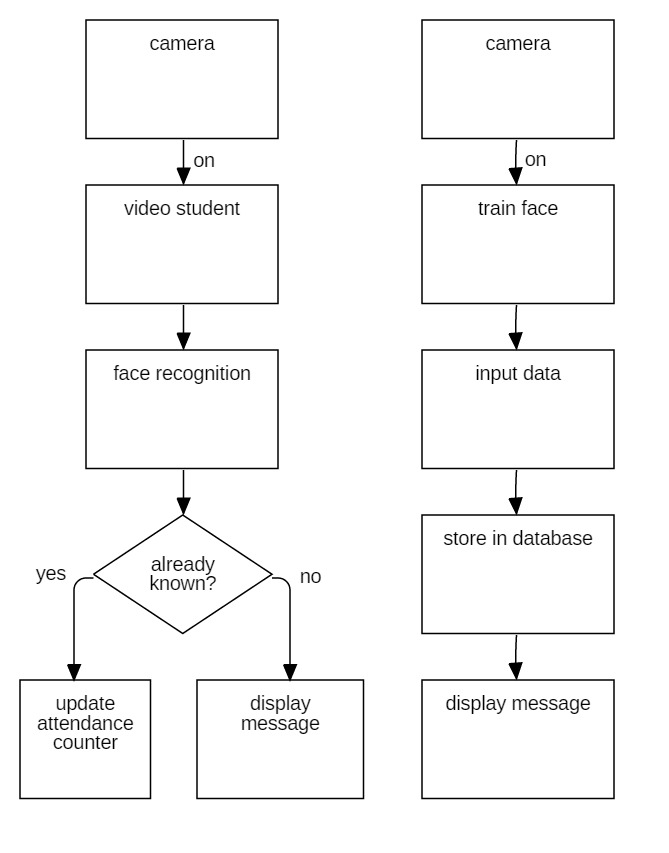
\includegraphics[width=1.0\columnwidth]{images/flowchart_diagram_whole_software}
	\caption{Flowchart showing the flow of the whole software.}
	\label{fig:folder}
\end{center}
\end{figure}

\subsection{Architecture}
The architecture is based on the Model-View-Controller pattern with three packages.
\subsubsection{GUI (View)}
This package consists of two classes: 
\begin{itemize}
\item MenuScreen: consists of the buttonclick methods for  Train, Options, and Exit. 
\item AttendanceScreen: When you click Start, menuscreen will create attendance Screen.
\end{itemize}

\subsubsection{Database (Model)}
This package consists of three classes:
\begin{itemize}
\item StudentModel
\item SqliteDataAccess
\item DatabaseController
\end{itemize}

More specifically inside the StudentModel class all students information are there like GivenName, LastName, matriculation number, and a list of images.
SqliteDataAccess class  is mainly used to connect the database for loading, storing,  and deleting students.
DatabaseController class should be used by the other packages for working with database. It calls the methods of SqliteDataAccess.
\subsubsection{Controller}
This package consists of four classes:
\begin{itemize}
\item Global
\item FaceAlgorithm
\item Camera
\item ClassifierTrain
\end{itemize}
More specifically Global class includes all static variables that need to be shared between classes.
FaceAlgorithm  class is mainly used to detect and recognize the face.
Inside the ClassifierTrain class we call the EmguCV’s algorithms. FaceAlgorithm class will call ClassifierTrain class.
By using Camera class we can take image from camera and show it in the GUI. 

\begin{figure}[H]
		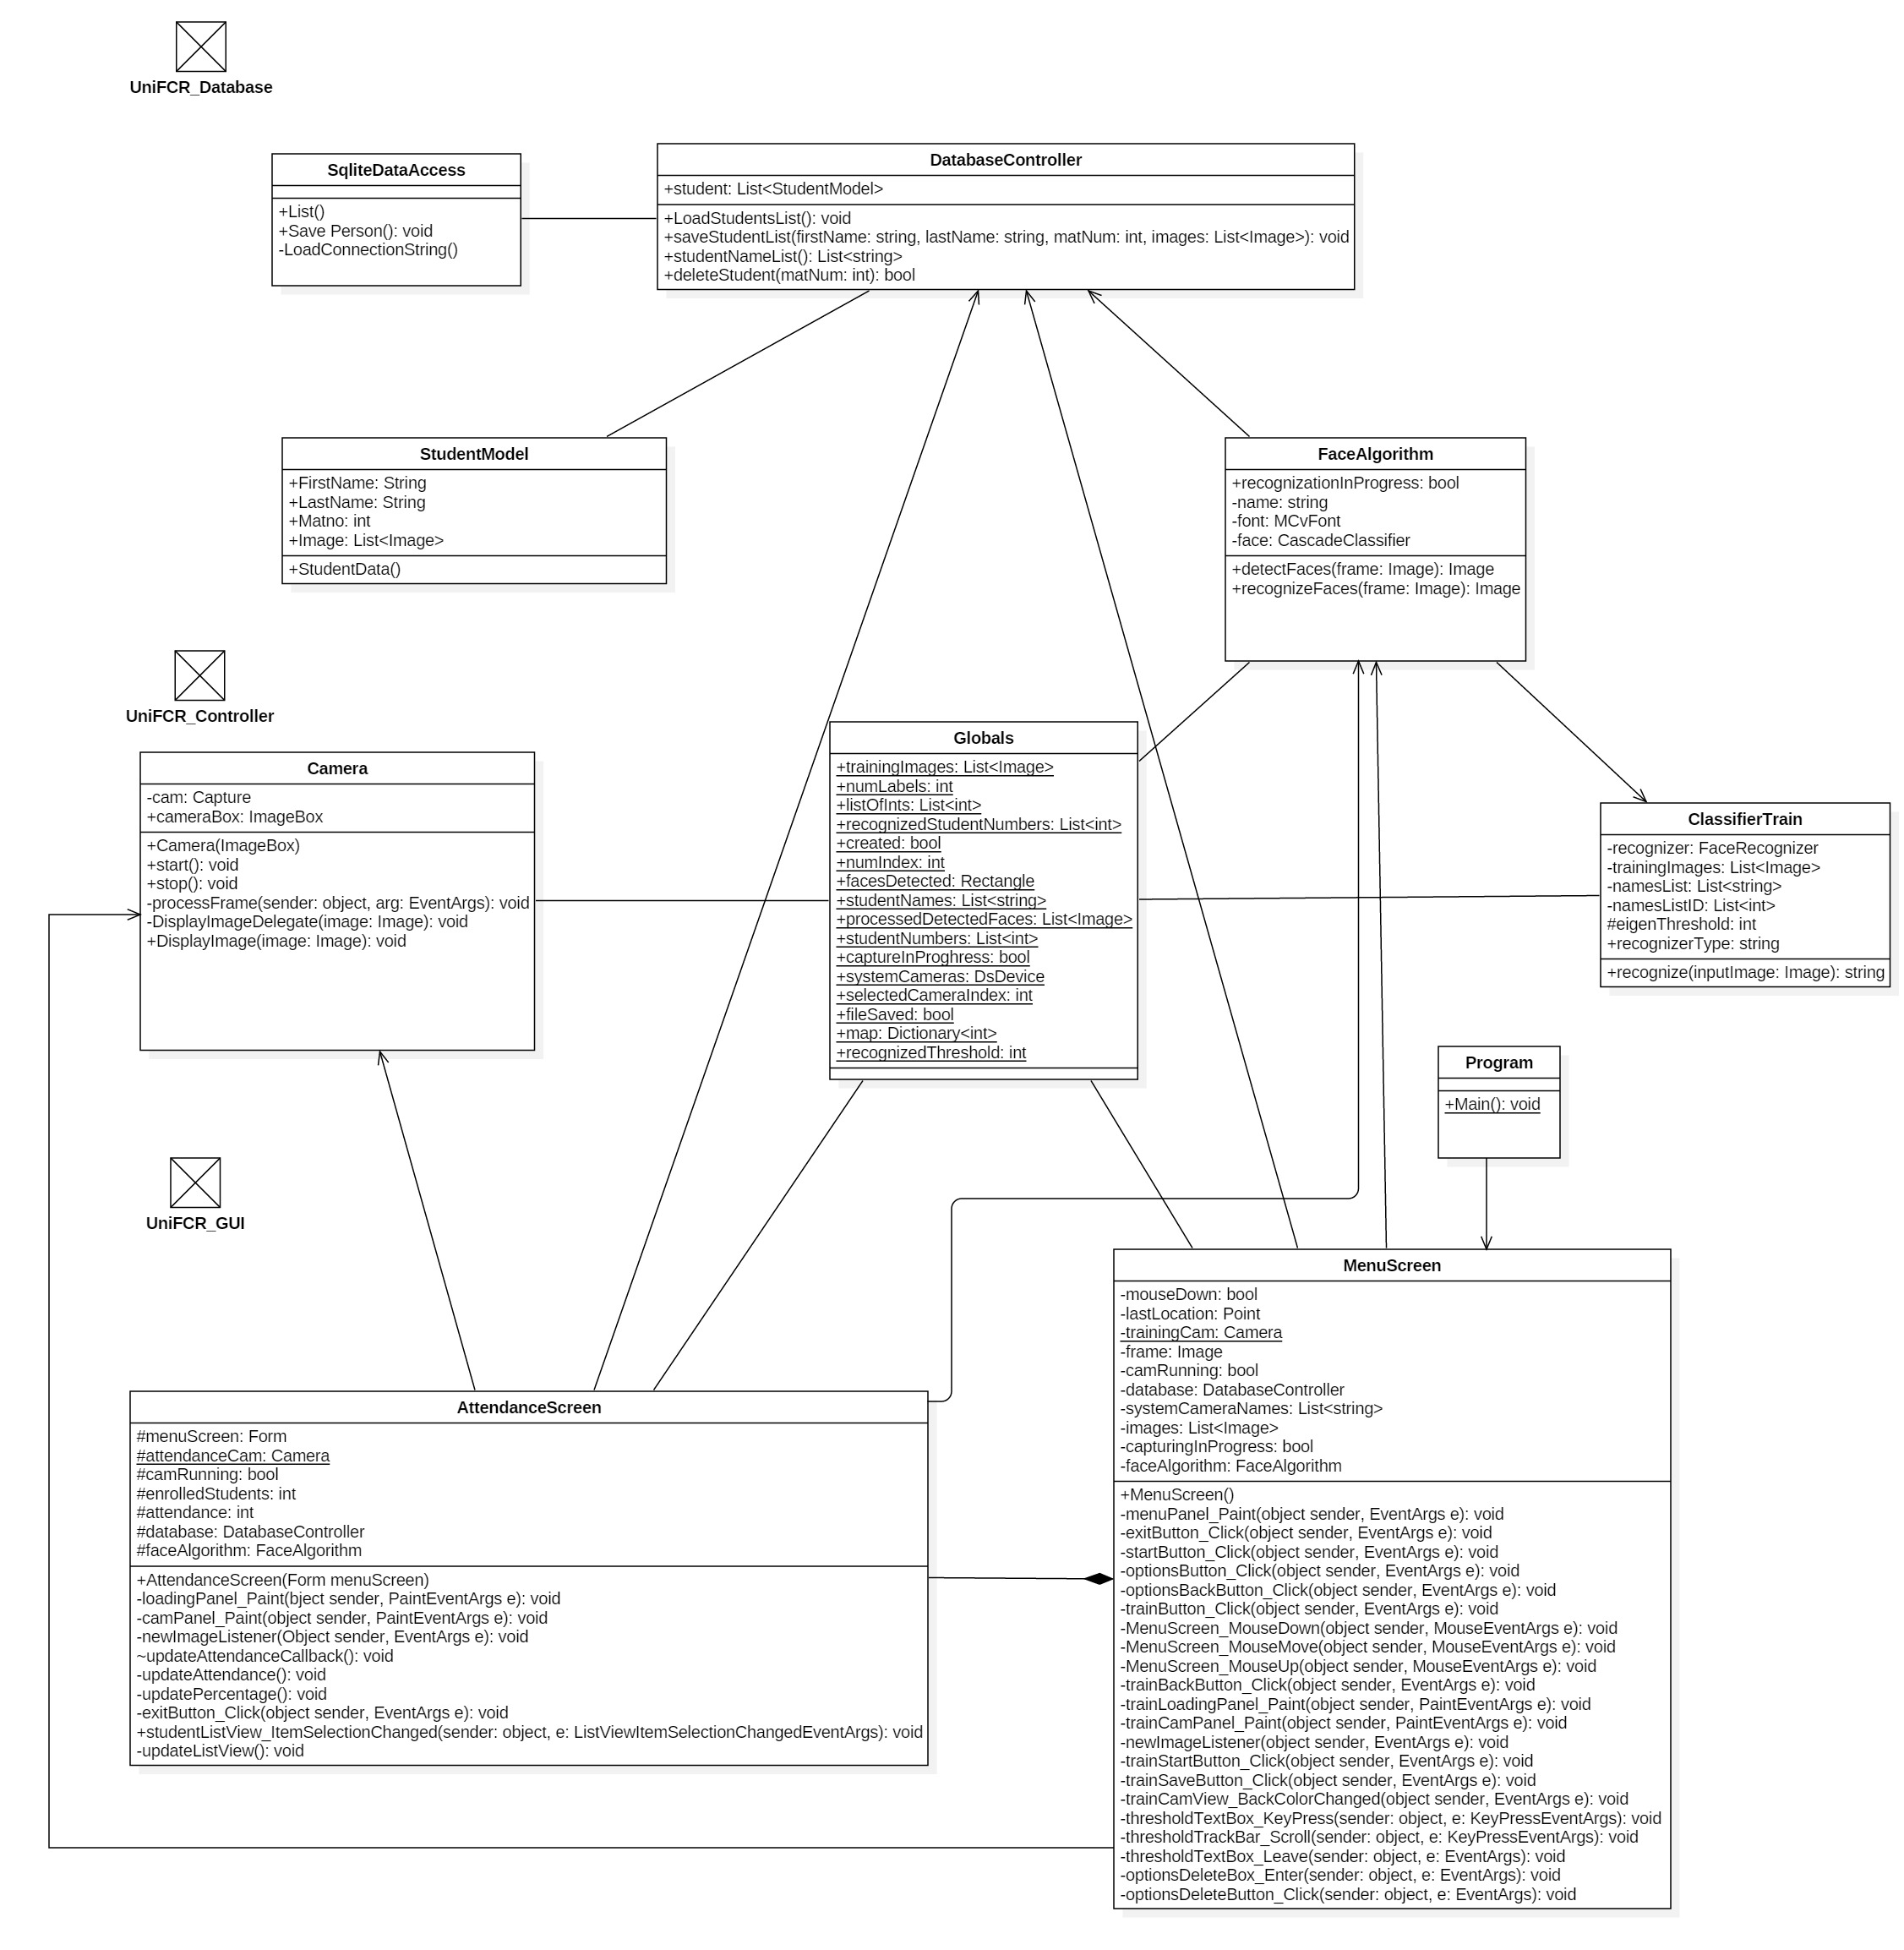
\includegraphics[width=1.2\columnwidth]{images/class_diagram}
	\caption{Class diagram showing all classes of the software}
	\label{fig:folder}
\end{figure}



\newpage



\section{Project Documentation}
\subsection{Process Model and Team Organization}
Our team followed the methodology of Scrum. In our project however, we didn't always stick to the same roles. We rotated the Scrum-Master a few times between Rahul Tak, Chisom Kobbe-Nwabufo and Florian Kessler. The development team consisted of Abbas Bushehri, Syed Habibullah, Lukas Heimann, Florian Kessler and Chisom Kobbe-Nwabufo. Within that development we created sub- groups and we ended up mostly doing pair-programming:
\begin{itemize}
\item GUI: Lukas Heimann
\item Algorithm: Abbas Bushehri, Florian Kessler, Rahul Tak
\item Diagrams: Syed Habibullah
\item Database: Chisom Kobbe-Nwabufo
\end{itemize}
We organized our typical working day from Monday – Friday from 9:00 am to 4:00 pm. One homeoffice day was included which switched from Moday to Friday. On homeoffice days, a group Skype-conference was held to discuss results and ideas. The day started with a daily scrum where we also made a to do list for the day. Next, we set the priority of each daily task and started working on them. Two retrospectives were held with the support of Dr. Balser where we discussed our successes and problems of the recent sprints. Organizing the Git repository was mostly done by Lukas Heimann and Abbas Bushehri. We created branches for each team member and had the most updated software version on the master branch.

\subsection{Planning Documents}
\subsubsection{Product Backlog}
\begin{enumerate}
\item As a professor, I would like to know who attends, because the course is mandatory
\item As a professor, I would like to receive an attendance counter on the amount of students attending, because I want to receive feedback on the popularity of my course
\item As a professor, I would like to see a live feed of the camera on screen, because it gives me an overview of the student group
\item As a professor, I would like to have an organized and neat GUI, because I want to navigate the program quickly
\item As a developer, I would like to make use of the full resolution of the camera, because the facial recognition works best with a high resolution feed
\item As a professor, I would like to get a visual name display about the students seen in the live feed, because I want to remember each student's name
\item As a developer, I would like to have a training mode, because I want to train the AI to recognize faces more accurately
\item As a professor, I would like to be able to choose the camera connected to my laptop, because one camera could get damaged
\item As a developer, I would like to have a slider for the eigen threshold, because I want to adjust the eigen threshold live to find a fitting value
\item As a professor, I would like to save all attending students as a list in a file, because I want check, which student attended my lessons in the course of a semester
\item As a professor, I would like to see a diagram that shows the attendance rate of the students in my lesson over the course of a semester.
\item As a professor, I would like to receive feedback on who stayed until the end of my lecture, because I want to have feedback on the quality of my lectures
\end{enumerate}

\subsubsection{Use-Case Diagram}
\begin{figure}[H]
		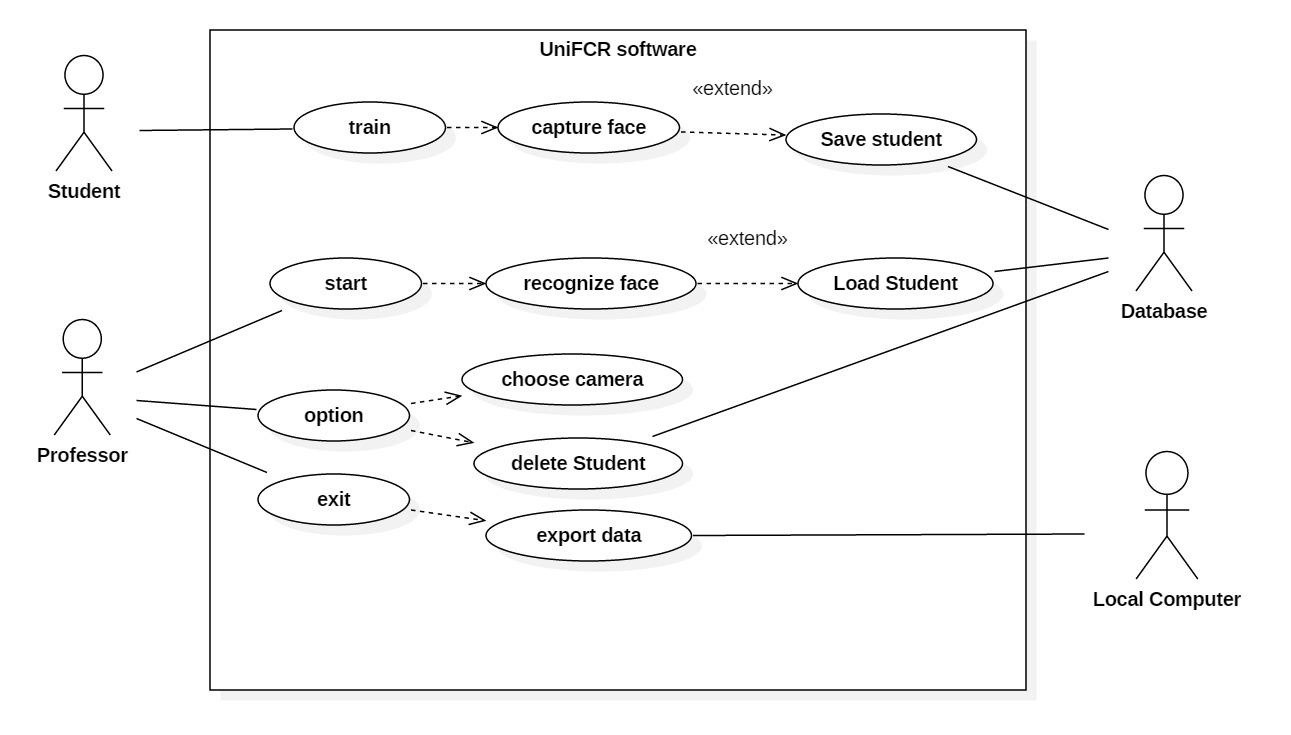
\includegraphics[width=1.2\columnwidth]{images/use_case_diagram}
	\caption{Use-Case Diagram}
	\label{fig:folder}
\end{figure}

\newpage




\section{Individual Contribution -  Florian Kessler}
\subsection{Research}
In the team-oriented project, I was mostly part of the algorithm subgroup. In the starting phase of the project, I gave an introduction of the basic functionalities of a supervised artificial neural network. In the following days, I did research about facial recognition algorithms and first found the Haar Cascade algorithm. After summarizing, finding a suitable way of implementing this method was the next important step. EmguCV in connection with OpenCV seemed like a suitable and practical possibility to create a facial recognition software.
\subsection{Organizational Responsibilities}
 To plan the sprints, I documented the tasks and managed Jira along the journey. Furthermore, I recorded every working session in writing in a separate document. Having been a Scrum-Master for two sprints, I was responsible for the typical organizing tasks in the project:
\begin{itemize}
\item holding the daily scrum
\item writing the to dos for the day on the whiteboard
\item prioritizing daily tasks
\item trying to help my team members if necessary
\item holding and documenting a retrospective with the support of Dr. Balser
\end{itemize}
\subsection{Algorithm}
During the sprints, I was mostly pair programming with Abbas Bushehri. Together, we implemented the Haar Cascade algorithm which we later extended to the Principle Component Analysis (PCA) method. In the \textit{FaceAlgorithm} class, we coded and used several components:
\begin{itemize}
\item\textit{CascadeClassifier}: contains a few XML files, depending on which facial recognition algorithm you want to use. We used the Haar Cascade file containing descriptions of the makeup of a frontal face.
\item \textit{detectFaces(Image\textless Bgr, byte\textgreater  frame)}: this method is called before the recognition method and used on its own in the train mode. Each frame of the live feed is converted in a gray scale image as an array of bytes. In the list \textit{Globals.processedDetectedFaces}, all the faces detected by the inbuilt\textit{DetectMultiScale} method of the \textit{CascadeClassifier} are saved. In the for-loop, the positions and dimensions of the red rectangles that are drawn in the GUI are calculated and the cropped images of the detected faces are added to\textit{ processedDetectedFaces}. In the end, the manipulated frame is returned to be used in the recognition method.
\item\textit{recognizeFaces(Image\textless Bgr, byte\textgreater frame)}: until the \textit{frame.Draw(...)} is being called, the method is the same as \textit{detectFaces(...)}. Since \textit{recognizeFaces(...)} is being used separately in the attendance (start) mode, we decided to copy the recognition part. The list \textit{Globals.trainingImages} contains all the images of faces saved from previous photo sessions. The \textit{Eigen\_threshold} is an int value that basically defines the threshold of the AI deciding to recognize a detected person as someone that's stored in the database or a stranger (unknown) and is set in an instance of the class Classifier\_Train. The image of a frame is handed over to this instance Eigen\_Recog for it to recognize the result (manipulated image of face of frame). The \textit{Eigen\_Recog} is now no longer needed and thus disposed. In \textit{Globals.map\textless int, int\textgreater}, the matriculation number of a recognized student is saved and the amount of frames he/she has been recognized in a live feed session. This is done in case faulty recognition occurs that would otherwise mark this student immediately as attended wrongfully. Because of that,\textit{recognizedThreshold} contains the number of frames a student has to be recognized in order to determine, whether he/she attends. If a person has not already been recognized and is known, a new entry is being made in the map with his/her matriculation and at first zero times recognized. Should the student already have an entry in the map and is being recognized again, his attendance counter increases. Lastly, the program checks whether the amount of time the student has been recognized satisfies the condition of the \textit{recognizedThreshold} and if it does, he is added to \textit{recognizedStudentNumbers}, which marks him/her as attended. A system access violation that occurred at times, when the live feed was displayed in the GUI panel, had to be caught.
\end{itemize}
\subsection{Debugging}
We encountered some more bugs, for example: the program would show weird errors and nullpointer exceptions which we couldn't make any sense of. This was fixed by upgrading from VisualStudio 2017 to VisualStudio 2019. After that, we separated the code in a more suitable structure to have the GUI and the algorithm in different classes. This however was just a temporary structure and was later significantly changed again.







\section{Individual Contributions - Abbas Bushehri}
\subsection{Webcam}
In the beginning of the project, we were given a webcam to use. However, after using it we determined that its quality was too low and the area it covered was too small. My laptop’s camera was better, but still not good enough. It was my task to pick a webcam that would meet the project’s requirements. I chose the C920 Pro HD Webcam. This webcam has a quality of 1080p and 30 FPS, and it comes with a wide angle. It could also be adjusted to mount on any laptop.

\subsection{FaceAlgorithm First Version}
I was then put in charge of programming the first version of the FaceAlgorithm class. This class would implement both face detection and face recognition using the Emgu CV library. I started by implementing the face detection method separately. Once that worked I moved on to writing a method that saved a student’s face along with their data. This method would be called in the training mode, whose GUI had just been completed. We were planning on saving this data in a database, however the database was not finished yet. So instead I had the method store everything locally in a folder for now. Then I wrote the method for face recognition in the FaceAlgorithm class. This method relied on the local folder as well. The method also required a class called EigenObjectRecognizer that I got from the Internet. This class implemented the Emgu CV algorithms. The face recognition method was used in both the attendance mode and the training mode.

\subsection{FaceAlgorithm with Database}
After the database was completed, I changed the FaceAlgorithm class to implement it. This included changing both the facial recognition method that needed to go through all the student images, and the class constructor. I also updated the method that saved the student data in training mode. This was all done in pair programming along with most of the team.

\subsection{FaceAlgorithm with Globals}
The team decided to implement a stronger architecture for the program. This lead to splitting it into three packages, one for the GUI classes, one for the database classes, and one for the controller classes. The FaceAlgorithm class belonged to the controller package. As a team, we made sure that FaceAlgorithm was no longer directly connected to so many classes. The problem was there were many variables that had to be shared between the FaceAlgorithm and GUI classes for the program to work. I came up with the Globals class to solve this issue. Globals is a static class filled only with variables. These variables are all static and can be accessed by any class in the program. We also changed the face detection and recognition methods. Now they took the camera’s frame image as a parameter and returned a frame after processing.

\subsection{PCA}
The face recognition method’s accuracy was not good enough. To improve this, Florian suggested we change the code to implement PCA and parallel optimization. Together we achieved this through pair programming. This lead to deleting the EigenObejctRecognzier class and replacing it with the Classifier\_Train class. Classifier\_Train implemented the improved algorithm we wanted. After implementing PCA, the program’s accuracy increased while the speed decreased. To fix this, we made the algorithm save and load the Eigen recognizer to a file instead of constantly initializing with the array of images. This did increase the program speed.

Florian and I noticed a variable in the algorithm called the Eigen threshold. After doing some research, we decided to test this variable to find the value that best fit our program. We had Lukas add the option to change the variable during run-time into the GUI. We then determined that the best value for the threshold was 2000.

\subsection{Threshold and Attendance List}
The team decided to implement a threshold for the attendance. If the number of times the student was recognized exceeded the threshold, then the student should be marked as attended. To implement this code I needed to add two variables to Globals. One of them is a dictionary where the key is the student’s matriculation number and the value is the number of times this student has been recognized so far. This dictionary should be updated every time the face recognition method is called. The second variable would be the threshold value itself. I wrote the code that implemented this threshold, and then Lukas added the option to set it in the options menu in the GUI.

After this, Rahul came up with the idea to save the list of students and their attendance in a csv file. This file would be written after the program is closed, and if the user clicks Yes on the message box that appears. We decided the file should be added to a Lists folder. The program should check if the folder already exists, and if not create it. Since the attendance should be taken daily, the name of the file should depend on the current date For example, attendance\_07\_11 would be the filename on November 7. Also, if a file with the current date already exists, then it will be overwritten, since the program should only be run once a day. Using pair programming, Rahul and I implemented the saving of the attendance list in the code.

\subsection{Error Handling}
During the project, there was a bug that I solved along with Florian and Lukas. The first was a system access violation exception. This error caused the program to crash randomly after returning to the main menu from the attendance screen. First we tried to use a try-catch but that didn’t stop the crashing. This error occurred because the FaceAlgorithm tries to return a frame after the attendance screen has already been closed. In the end, the best solution we could find was to call Thread.sleep(1000) before the attendance screen is closed and disposed. This makes the attendance screen wait one second. This is enough time for the FaceAlgorithm to return the last frame to the attendance screen and avoid this error.



\newpage



\section{Individual Contributions - Rahul Tak}
In the team oriented project, I was mostly for organisational and algorithm part of the project. In the first week, the project planning was one of the task that I took responsibility of. Like setting up the dates, meeting points, sprints etc. Also I was the scrum master and I took responsibilities of everyday sprints and Backlogs. I took over the responsibility for designing the Vision document and milestones for the team to achieve in the coming weeks.

The idea which I gave for the pair programming worked really good for our team. So I decided to give every individual a single main responsibility and then I sub divided the group into small teams of two people. This approach worked wonder for us. 

During some specific tasks, I was paired with Habib for Documentation, was paired with Abbas for Algorithm. 
\begin{itemize}
\item Vision Document
\item Milestones 
\item Scrum 
\item Project Planning 
\item Algorithm Research 
\item Creating CSV file
\item Poster Designing
\item Presentation 
\end{itemize}



\newpage



\section{Individual Contributions – Lukas Heimann}
I had two main responsibilities during this project. The first one was creating a good looking, easy to use, modern user interface. The other one was to write the Camera class that contains all the methods to grab frames from the webcam and then later display them in the GUI.

For the GUI I went with a modern, flat UI design. The main colors of the interface are white and blue, to also match the general design of the THU. I created our Logo with free icons from www.flaticon.com.\cite{Logo1} \cite{Logo2} All of the GUI elements are borderless and flat to give the interface a modern look and feel. We didn’t want to have too many different windows for the different parts of our software (main menu, options, attendance mode etc.). Therefore, I used only one form to display the main menu, options menu and training menu.

\subsection{Main Menu}
The main menu contains 4 buttons.
\begin{itemize}
\item Start: starts the attendance mode
\item Options: shows the options menu
\item Train: shows the training menu
\item Exit: closes the window and saves the attendance list as a .csv file
\end{itemize}

In the options menu there is a dropdown list containing all cameras that are connected to the computer so the user can choose which camera will be used in the attendance mode. Also, there is a text box where the user can enter a matriculation number. If they then press the \textit{Delete} button the student with the matching matriculation number will be deleted form the database. 

The training menu is used to enter students in the database. First, the user can enter a students name and matriculation number.  When the user presses the \textit{Capture} button the software captures ten images of the face in the view of the camera. The images are only captured if the algorithm detects exactly one face in the frame. If they then press the capture button again the software captures ten more images. After enough images have been captured the user can press the \textit{Save} button to then save the data in the database. 

\subsection{Attendance Screen}
This is the second window and the main part of our software. It contains the camera feed as well as the most important information for the professor.

\subsubsection{Camera Feed}
As our idea was to show the names of the students in the camera feed to help professors and lecturers remember the students names, I use a full screen window for the attendance screen. This way I get as much space as possible for the camera feed. The panel that shows the camera takes up 3/4 of the screen but the aspect ratio of the camera is preserved (16:9) so the picture doesn’t look stretched.
 
\subsubsection{Side Panel}
The camera feed taking up 3/4 of the screen gives us enough space to put a sidebar on the right-hand side that contains the most important informations for the professor. At the top of the side panel there’s the UniFCR Logo. Then we have an percentage counter that shows the percentage of attended students. For this I decided to use a circular progress bark. This creates a modern look and also gives a good visual feedback to the professor who wants to see how many students are currently attending the class. Right beneath that we have a label that also shows the total number of students who are currently attending the class. The last part of the side panel is the student list. This list contains all students that are enrolled in the course (in our case all students in the database). If a student is marked as attended the background color of their table entry changes to give a visual feedback to the professor which specific students are currently attending the lecture. I first wanted to show the full information about the student (first name, last name and matriculation number) in this list. But then the list was too big to fit in the side panel creating unwanted scrollbars. I tried to make the list scrollable by dragging the mouse to hide scrollbar from the UI but in the end this didn’t work out. So, I decided to just show the names of the students which made the list significantly smaller. 


\newpage



\section{Individual Contributions - Chisom Kobbe-Nwabufo}
\subsection{Research}
In the team-oriented project I was responsible for the Database implementation. My Team and I initially decided on using MYSQL database. I researched of what type of database that is most suitable with our type of project. From my research, I came to conclusion the SQLite database would be the best for project.
SQLite is a library that gets embedded inside the application that makes use of it. SQLite being a self-contained, file-based database that consists of a single file on the disk, it makes it extremely portable and reliable.

\subsection{Dummy GUI and Database}
In this stage, after deciding the goal of our project. I made the first sketch, design and implementation of the GUI which together with the \textit{dummy} database later served as the \textit{dummy} samples to the team. Because the main GUI was still under development by Lukas, to test the database class and functions like the \textit{load} and \textit{store} functions I implemented I made of the \textit{dummy} GUI and database. 

\subsection{Database}
I first implemented the database to contain as the data (Student names, Matriculation number and multiple images of each student) in one table. This was a bottle neck, difficult and did not support the \textit{Normal form} in DBMS. I then updated the database for data (Student names and Matriculation number) to be stored in one table(Student table) and then the images stored in the Image table using the matriculation number as the Primary key. The Image table consists of an autoincrement column, Matriculation number column and Image column which contains 70 images per student stored in the database.
To access the database I implemented the \textit{SqliteDataAccess} class which contains methods like \textit{LoadConnectionString()} which gets the connection string of the SQLite, \textit{LoadStudents()} -this method returns the list of students in the database, the \textit{DeletePerson()} method takes a matriculation number of a student from the textbox and deletes it from the two tables(Student and Image Table) in the database, \textit{SavePerson()}- saves the \textit{GivenNames}, \textit{LastNames}, \textit{MatNo} and Images of just one student per access/connection to the database.

The \textit{DatabaseController} class worked as the business/logic component for the database. The \textit{StudentModel} is a simple class which just contains a basic declaration of the student data- \textit{GivenNames}, \textit{LastName}, \textit{MatNo}, image and a \textit{StudentData} method that returns the student’s information without images.

\subsection{Error Handling}
I encountered “Insufficient parameters supplied to the command” error while saving data to the database. I solved this by creating a different query for inserting into the Image table while still using the same connection to insert to the Student table. This was possible because the MatNoID in the Image table is a foreign key to the MatNO which is a primary key in the Student table.



\newpage



\section{Individual Contributions - Syed Habibullah}
In the team oriented project I was mostly part of the diagram part and  some of the documentation stuff.

\subsection{Class Diagram}
How the class diagram helps our project:
\begin{itemize}
\item For example, a UML class diagram showing all the classes on a package, with all their attributes and methods --something that can be easily auto-generated-- provides no value at all: it is at the same level of abstraction than your code. Plus, the code will most surely be a better source for that information because it will always be up to date, and it will probably be documented and organized in a way that is easier to know which methods/attributes/things are more important.
\item On the other hand, if you have concepts of a higher level of abstraction than what can be expressed expressed on the code, documenting those on a diagram can be a good idea. 
\item For example, a diagram showing the higher level abstract modules on a complex system, with their dependencies and maybe a little description of their responsibilities and what package/namespace they map to in the source-code can be a really useful for a new team member that needs to be introduced to the project, or can also be used to figure out where a new class/functionality should be thrown.
\end{itemize}

\subsection{Use Case Diagram}
How l use cases help us to manage our  projects?
\begin{itemize}
\item \textit{Scope}: The use case diagram is a particularly effective tool to help identify and manage the project scope. Although only being one of the many aspects of project management, scope management is often considered the most difficult. The use case diagram helps to identify the scope in these ways:
   \begin{itemize}
     \item Sets the boundary for the project. The boundary box indicates the scope of the system. Everything within the box is included in the system; anything outside of the box is excluded. This diagram is a wonderful graphical representation of system scope.
     \item The flow of events confirms the scope. It provides the details involved with each use case process and describes how big each process is.
     \item All the use cases need to link to the business and project vision and objectives. Any use case that does not provide this alignment, can be easily seen and removed.
     \item Showing system actors helps provide a picture of the interfaces that need to be modified. This picture aids in showing not only what's contained in the application, but also how many system interfaces need to be included in the project. It provides an effective communications tool and visual that may be helpful in explaining and estimating the effort that may be transparent to business customers.
   \end{itemize}
\item The use case diagram helps to control the scope in these ways:
   \begin{itemize}
     \item Once use cases have been confirmed, new use cases that arise can be better managed. Changes can be matched to the vision and original diagram to see whether or not they belong. New requests can be translated into new use cases and placed in the diagram.
     \item If new actors surface, it is an indication that more work is required. Again, the visual serves as a way to communicate with business experts about the impact of their requests on the project.
     \item If new use cases cause any linkage to change, additional work will be needed as well
   \end{itemize}
\end{itemize}



\newpage


\section{Retrospective}

\subsection{Goals Achieved}
\begin{itemize}
\item  modern, easy to use GUI
\item  database integration successful
\item  generated attendance list
\item  successful implementation of detection and recognition algorithm
\item  training mode adding several pictures per person works
\end{itemize}

\subsection{Lessons Learned}

\begin{itemize}
\item  plan more time for research
\item  C\# not best choice for face recognition, use Python instead
\item  be more careful when merging code in Git
\item  how to use branches in a project like this in Git
\item  more efficient project management with Jira
\item  basic understanding of functionality of face recognition
\end{itemize}

\subsection{Problems}

\begin{itemize}
\item  Moral question: Should you use such a software? Is it ok to do this?
\item  Difficulties getting training data
\item  Privacy issues: who would want to give pictures of themselves?
\item  Faces of people with dark skin not recognized well
\item  Low frame rate due to algorithm setup
\item  Github
\end{itemize}

\begin{itemize}
\item  Mistakes when merging
\item  Difficulties pulling latest code
\item  Formulations of tasks too vague
\item  Time estimations were off
\end{itemize}



\newpage




\section{Outlook}
In general, we are really satisfied with the result of our project. As we mentioned before, our software is more of a proof of concept that shows that this idea could actually be used to replace an analog attendance list on paper. But there are still some problems that need to be fixed first and functionalities that could be improved. 

\subsection{Problems}
First of all, there is the problem with the training data. We need a way to get enough pictures of all students in the course so that the software can accurately recognize them. A possible solution would be to make an app for students that allows them to capture training data for the database themselves. Also, there is the problem with the inaccuracy of the recognition. To fix this problem we would have to implement a better neural network and train it with more pictures. Also, we could  try to use negative training data to further improve the accuracy. Another problem-solving approach would be to normalize the pictures captured in the training mode to possibly increase the accuracy of the detection. 

\subsection{Improvements}
There are also some functionalities that could be improved in the future. One idea would be to collect more data about the students attendance. For instance, we could save the times when students were first and last recognized. That way the professor can also know if a student was late or left early. Another idea would be to automatically message the missing students to remind them that they need a medical certificate. It would also be useful to add more options to the options menu so the professor can for instance change camera settings like: resolution, framerate, brightness, contrast, etc. 
\newpage
\bibliography{References}

\end{document}